\chapter{Packet Processing}
\label{chapter:packet-processing-systems}

Packet processing refers to the methods and concepts applied to transport data packets through the various network elements in a communication network. The network routers, switches, and other devices, such as computers and smartphones, all have their own packet processing subsystems to manage the packet traversal between the network elements. This thesis focuses on the packet routing equipment in the middle of Internet backbone.

This chapter presents the general methodology of packet processing and network processing units. We begin by describing the general packet processing framework used in network processors. After that, we present the packet flow handling and quality of service methods, emphasizing the importance of packet buffering and queuing theory in the packet processing. Further, we present an overview of the hardware architecture and programming models used in packet processing units.

Finally we will have a closer look on a specific network processing unit, Cavium OCTEON II CN6880, and instrument the system to obtain the required information to model the system. Two different measurements will be done: one to measure the communication latencies, and another to measure the memory latencies and throughput.

\section{Packet Switched Networks}
\subsection{Network Components}
Packet switching refers to a method of transmitting data in separate, suitable sized blocks, called packets, between the links of a telecommunications networks. The importance of packet switched networks is increasing in every part of the communication networks, which is explained partly by the Internet itself being an enormous packet switched network.

The Open Systems Interconnection (OSI) model is a standard conceptual model, which characterizes the communication functions involved in a general network communications of computer system. The model defines seven hierarchical layers of functional elements, between the physical interconnections (layer 1) and the software applications (layer 7).~\cite{ISO:1994:OSI}

The Internet Protocol Suite, or Transmission Control Protocol / Internet Protocol (TCP/IP), is a set of core protocols for the Internet and similar packet switched networks. It provides end-to-end data communication and specifies data packetizing, addressing, transmission, routing and receiving in the packet network. In addition to TCP and IP protocols, it provides several other network and transmission layer functionalities. The functionalities are divided into four abstraction layers: application layer, transport layer, internet layer, and link layer.~\cite{Braden:1989:TCPIP}

Internet Protocol (IP) is an essential Internet layer protocol of the Internet Protocol Suite. It provides the necessary addresses and (unreliable) delivery mechanisms for datagrams between the transmission endpoints. It is a connectionless, best-effort protocol with no error control, sequencing, or end-to-end reliability, but rather contains only the functions for packet fragmentation and delivery through the network. The packets in the IP protocol can be forwarded independent of other packets, forwarding them on-the-fly by routers.~\cite{Deering:1998:Internet}

A packet refers to the unit of data transmitted across the network. Packets consist of two parts: the header information and the payload data. Network routers use the header information to direct the packet to destination system, whereas the payload is extracted and used by the application software. All the higher layer protocols in the TCP/IP stack are encapsulated in the IP-packet's payload section.~\cite{Deering:1998:Internet}

In a conventional IP-based network architecture, the packet processing equipment and functionality is partitioned into three components: management plane, control plane, and data plane.~\cite{Chao:2007:HPS}

The control plane refers to the parts of the routing architecture, which carries and consumes the control packets needed to describe the network topology and correctly route the actual data packets. The control packets originate from and are destined for a router.~\cite{Chao:2007:HPS, Yang:2004:FCE}

The data plane, often referred as forwarding plane, deals with the actual data forwarding in the network. It defines the part of the routing architecture, which decides destination and takes action for the data arriving to it. The decision is typically determined by a look-up table, which the incoming packet is compared to. The management plane carries the traffic used for the administrative tasks of the network.~\cite{Chao:2007:HPS, Yang:2004:FCE}

\subsection{Traffic Characteristics}
The nature of the high-speed packet processing entails new types of constraints to the computing; Advanced stream processing systems are needed to process the data on-the-fly in the vicinity of the sources.~\cite{Bonomi:2012:Fog}

In the traditional von Neumann model of computing~\cite{Neumann:1993:EDVAC}, the computation is carried out by modifying the data stored in memory. However, the growing volumes of data and strict latency requirements, require not only distributing the computation, but also changes the nature of it more towards stream processing. The manipulation of the data streams passing through the system must often be done on the on-the-fly.~\cite{Bonomi:2012:Fog, Thies:2002:StreamIt}

In packet switched networks, the data streams are called \emph{flows}. Flows represent the data in specific time periods between specific network end-points. A single flow contains a large number of packets. The Internet Protocol allows each individual packet of a stream to be processed in any order, leaving the ordering of the packets to the end devices. This characteristic makes packet processing applications look like ideal for a parallel computing. However, protocols such as TCP/IP (accounting over 80\% of the Internet traffic~\cite{Fraleigh:2001:Packet}), have significant performance reductions due to reordering of packets in a single stream. For this reason, the packet processing systems often have built-in schemes, such as specialized queue management and buffering, to efficiently keep flow specific packets traversing through the queues in order.~\cite{Govind:2008:PacketReorder, Kumar:1998:RouterArchitecture}

\section{General Packet Processing Framework}

A general packet processing framework consists of three primary aspects: packet processing functions, packet direction (ingress, egress, or combination of both), and packet processing paths. These three aspects are depicted in Figure~\ref{fig:general-packet-processing-framework}. The packets enter the system from the left, from the physical line interface (ingress direction), and follow either the slow or the fast path. The packets are then forwarded either to the switch fabric or back to the physical line interface (egress direction).~\cite{Giladi:2008:Network}

\begin{figure}[]
  \begin{center}
    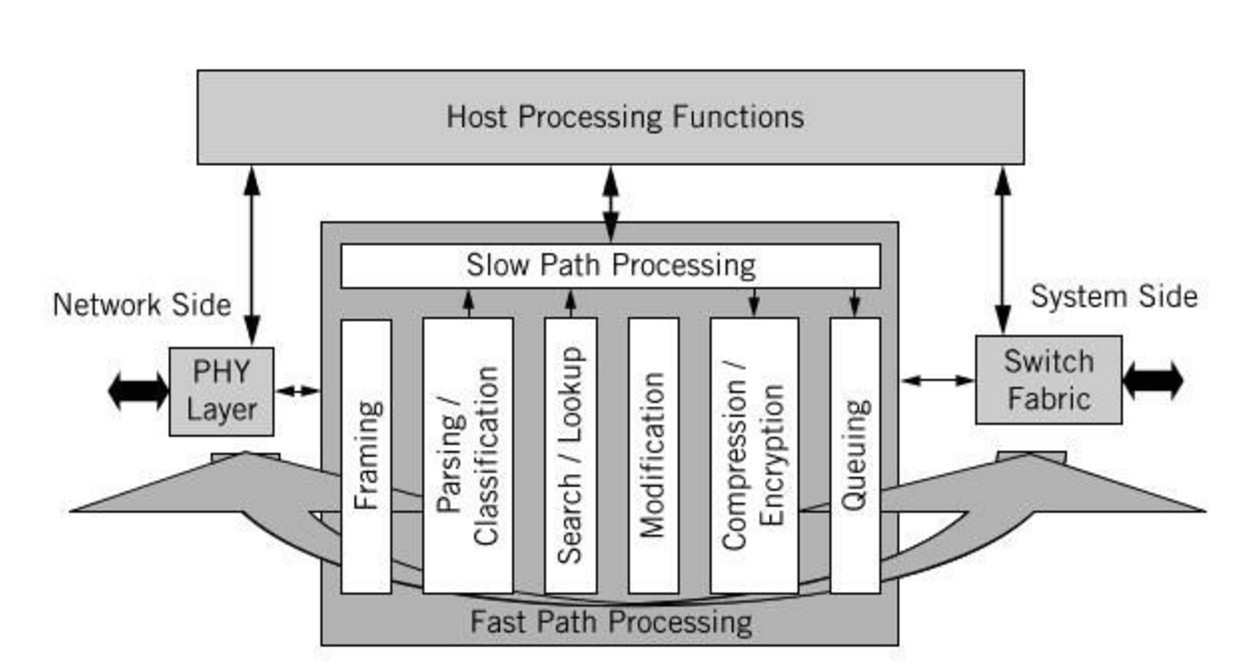
\includegraphics[width=\textwidth]{images/general-packet-processing-framework.png}
    \caption{A general packet processing framework. Figure from~\cite{Giladi:2008:Network}}
    \label{fig:general-packet-processing-framework}
  \end{center}
\end{figure}

\subsection{Ingress and Egress}
Ingress and egress refer to the packet processing done for the packets entering the network processor from the network, or packets leaving the network processor to the network, respectively. Ingress and egress processing, although not necessarily being clearly separated in modern systems, play an important role in the network processing units. The unclear separation of these phases is due to the various different implementations in today's network processing units. Some processors have one processing direction, from packet input to its output, possibly happening through the same interface. Other implementations might not have distinguishable elements that target ingress or egress processing.~\cite{Giladi:2008:Network}

Figure~\ref{fig:ingress-egress} outlines the basic two-part equipment implementation scheme, called half-duplex, for packet ingress-egress processing. The first part of the picture depicts the line cards for receiving/transmitting the packets from/to the network. The second part consists of switching fabric, service cards, and other processing functions and mechanisms that packets go through internally.

\begin{figure}[]
  \begin{center}
    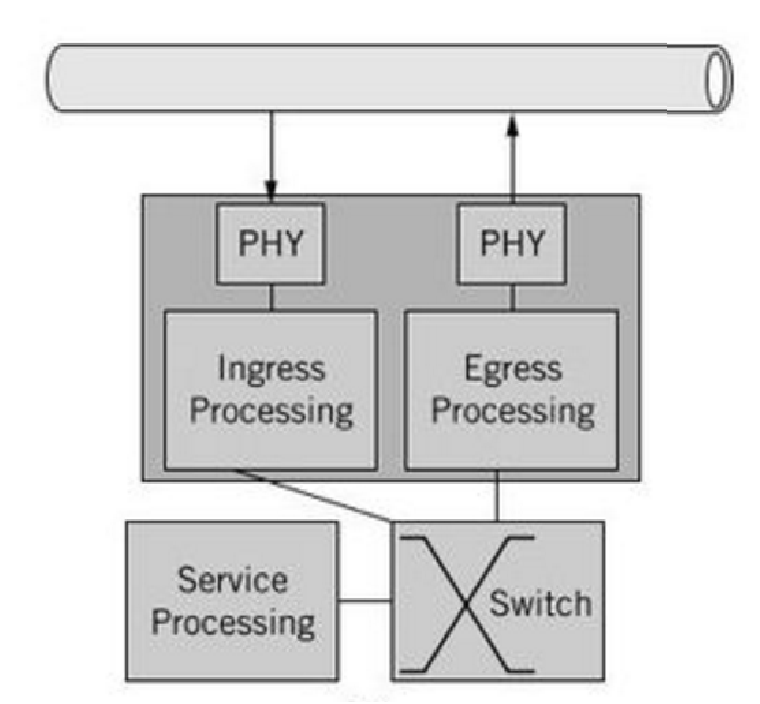
\includegraphics[width=.6\textwidth]{images/ingress-egress.pdf}
    \caption{Two part ingres-egress scheme. Figure from~\cite{Giladi:2008:Network}}
    \label{fig:ingress-egress}
  \end{center}
\end{figure}

Half-duplex processing consists of two dedicated processors for each direction. The functions executed on the ingress packets and egress packets can be distinguished, in which case the network processing unit often consists of separated processing paths for the two ways. Typical ingress processing tasks consists of, for example, error checking, classification, traffic management, header manipulations, and prioritization and queuing. Packet egress tasks, on the other hand, include checksum calculation, address lookup, packet forwarding, segmentation and fragmentation, traffic management, and packet prioritozation and queuing.~\cite{Giladi:2008:Network}

\subsection{Processing Paths}
In many cases, the packets flowing through the network processing unit need to be processed at wire speed, meaning that the number of packet leaving and arriving the processing unit must be equal at certain time interval. The introduction of increasing Ethernet speeds imposes strict constraints for the network processors. While the control- and management plane traffic can often be processed with fairly non-trivial solutions, the main bottleneck, to keep up with the scalability of optical transmission technology, is the data plane processing.~\cite{Giladi:2008:Network}

The comparison of the speeds of Ethernet based transport networks and the processor speeds gives a perspective of the packet processing requirements. A typical Ethernet link in the network backbone, with 100Gbps speed and minimum frame size of 64 bytes, leaves the packet processing system 6.7ns to process each packet.~\cite{Giladi:2008:Network}

Even in the most trivial packet processing applications, this processing requires several different processing steps. For each packet, the network processor must execute complex packet parsing, to parse destination address and port. Then, based on this information, the processor executes several searches to retrieve the destination details from the memory, possibly containing hundreds or thousands addresses. It is evident that completely software based slow path solutions are insufficient to answer these requirements.~\cite{Giladi:2008:Network}

Fast path architecture refers to a path through a computer program, which incorporates smaller number of instructions or other optimization methods, compared to the normal path. In packet processing systems, the vast majority of packets require very little processing. Thus, the data processing is often split into two, referring to the data plane and control plane processing: fast path and slow path.~\cite{6wind:2016:FP, Giladi:2008:Network}

The typical slow path of the packet processor is run on top of an operating system stack. The fast path layer processes packet outside the operating system environment, often with hardware acceleration, thus avoiding the overheads occurring from the thick software stack. This leaves only a small number of packets that require special processing, to be forwarded to the slow path able to do more complex processing. Typical examples of slow path packets in IP network are IP options and ARP packets. In MPSoC packet processing systems, such as Cavium OCTEON II CN6880, the processing cores can often be dynamically configured to run fast path or slow path~\cite{cavium:2010:fundamentals}.~\cite{6wind:2016:FP, Giladi:2008:Network}

\subsection{Packet Processing Functions}
Packet processing functions are separate tasks, following each other, in the packet processing path of packet processor. These functions can be categorized, for example, as framing, parsing and classification, search/lookup/forwarding, packet modification, compression and encryption, and queuing and traffic management.~\cite{Giladi:2008:Network}

The packet processing starts with the packet entering the network processor through the network interface controller's ingress port, immediately followed by the packet \emph{framing}. Framing assures that packets or datagrams can be correctly extracted from the incoming data frames. The incoming data frames are tested for correctness, to make sure all the bits in the frames are received correctly. If necessary, the framing functions attempt to fix the bits of the incorrect frames. Finally the integrity of the frames is validated, to make sure that all the packets' content arrived correctly.~\cite{Giladi:2008:Network}

Framing is done similarly in the egress direction, in order to assure correctness of out going packets. In the outgoing framing phase, the needed headers are attached or modified, proper terminals and trailers are added to the packet data, and error detection and correction information is appended.~\cite{Giladi:2008:Network}

After framing, the packet is \emph{parsed and classified}, meaning that the network processing unit inspects the packet data in order to understand its type, and then classifies it according to the application requirements. Parsing and classification are two combined subtasks, sometimes carried out either separately or together, depending on the system.~\cite{Giladi:2008:Network}

Packet parsing can be very simple and trivial, or it can be a complex task requiring unique language to describe and dedicated hardware to execute the process. Parsing means of identifying the relevant fields in the incoming data packet. These field's values are then used for either further packet parsing or classification, which is why these two are sometimes tied together.~\cite{Giladi:2008:Network}

Classification refers to the functions that categorize the packets into separate flows, by the rules defined in the system. Each packet belonging to a specific flow, then take the same processing steps. Packet classification can be stateful or stateless, static or dynamic, and the fields to be classified have variable of fixed lengths and offsets. In stateless classification, the decision is made solely based on the packet content, independent of other packets. In stateful classification, the system state changes based on the processed packets, and affect the classification decisions. In static classification all the classification criteria are predefined, and the rules are fixed. In dynamic classification, on the other hand, the classification criteria and rules are computed based on, for example, incoming packet or system's state. Packet classification can be implemented in hardware or software, depending of the required complexity.~\cite{Giladi:2008:Network}

\emph{Search} and \emph{lookup} functions are not packet processing phases themselves, like the other discussed packet processing functions. Rather, they are atomic operations used during the packet processing, such as classification, \emph{forwarding}, or any other phase. Almost every packet processing activity starts with an IP-lookup, thus making the search and lookup functions are probably the most important packet processing operations, in terms of effect to processing speed, in packet processing. Various different solutions, often referred to as ~\emph{search engines}, have been developed to enable searches at wire speeds. Search engines are software processes or hardware solutions, often packed in a separate co-processors.~\cite{Giladi:2008:Network}

% Packet classification and related memory searching are of main importance in processing, that are often implemented with special co-processors and parsing and classification languages.~\cite{Giladi:2008:Network}

In the \emph{packet modification} phase, the network processor drops or modifies the packet being processed, or possibly generates new packets as specified by the application. Packet modification is one of the key operations in many packet processing applications, especially in the ones other packet forwarding. Packet modification phase is also used for some traffic analysis, management and statistics collection tasks.~\cite{Giladi:2008:Network}

Some packet processing systems \emph{compress and encrypt} the packets before they leave the system. Compression and encryption are often done in the access network processors, whereas in the trunks of the network core, the packets just flow through. Compression is typically used in networks and applications where the bandwidth is limited, and security is used for privacy, data integrity, and authentication purposes.~\cite{Giladi:2008:Network}

Finally, in the packet transmission phase, \emph{queuing, prioritization, and traffic management} are used to make sure the traffic patterns are as expected. The traffic management process forwards the packets to appropriate output queues and schedules them for transmission, according to the line and receiver conditions, and the parameters, such as priorities, of the packets. Traffic management is also used to meter the packets, and transmit the packets on a desired rate and burstiness. Due to the complexity of traffic management, it is often implemented by a dedicated traffic manager co-processor. In some cases, packets incoming to the system also go through a traffic management phase.~\cite{Giladi:2008:Network}

% \section{Fast path Architecture}
% Commodity software and multi-core hardware can reduce the cost and provide high flexibity in the development and management of software packet processing, while at the same time achieving the performance of traditional hardware routers. This is achieved by replacing the thick software networking stack of commodity operating systems with special driver and kernel improvements.

% \section{Packet Flow Handling, Queues, Buffers}

% \todo[inline]{Packet Flow Handling, Queues, Buffers}

\section{Processing Hardware}
\label{sec:hardware-architecture}
% \section{Network Processor Architecture}
% TODO: http://ieeexplore.ieee.org.libproxy.aalto.fi/stamp/stamp.jsp?tp=&arnumber=668286
% Papaefstathiou:2005:Queue
% TODO: https://hal.archives-ouvertes.fr/hal-00181832/document
% Kumar:1998:RouterArchitecture

% high performance and programmability are competing goals
% -> even mutually exclusive?

% One of the cornerstones of the Internet is the ability to connect devices together into networks, and further set of networks into internetworks. Packet switches and routers ...

% Routers and switches are the cornerstones of the Internet. They are used to connect multiple heterogeneous devices together, forming a network of devices, whereas the routers connect. heterogeneous networks into internetworks.

Traditionally, the focus in the development of network equipment -- switches, routers, and various other middleboxes -- has been to achieve high performance with very limited packet processing functionalities. The network appliances and middleboxes have typically been deployed on special purpose Application-Specific Integrated Circuits (ASIC) hardware, mainly due to high performance requirements compared to the hardware development and the absence of extensibility and flexibility requirements.~\cite{Dobrescu:2009:REP}

However, the required network functionality is becoming increasingly sophisticated. In addition to the traditional layer 2 and layer 3 routing and switching tasks, the network elements are required to handle more demanding tasks (e.g. application acceleration, encryption, and intrusion detection) all the way to layer 7. These extensions often require modified per-packet processing on the router data plane, and as the specialized network processors are difficult to extend and program, both industry and research are seeking new, more flexible networking solutions.~\cite{Egi:2009:PP, Dobrescu:2009:REP}

On the other extreme of the design spectrum, are the software routers built from general-purpose operating systems and x86 hardware platforms. The main promise of the software routers is their extensibility in the software and hardware development: the system's network functionalities, both in the data and control plane, can be modified fully by the software, thus mitigating the hardware design and development burden of the network developers.~\cite{Dobrescu:2009:REP}

The software routers also enable several other properties of the general purpose computer ecosystem. Huge manufacturing volumes and widespread supply and support chain allow much cheaper hardware prices. The rapid advances in commodity semiconductor technology, such as the state-of-the-art power management features, can provide significant advantages over the slow hardware upgrade cycles of the traditional ASIC based systems.~\cite{Dobrescu:2009:REP}

The challenge with the full software routers is the scaling the approach to high-speed networks. Between these two extremes exist design solutions, which offer much of the programmability of commodity hardware and the performance of specialized ASIC systems. Our focus in this thesis, is on the MPSoC systems consisting of these middle ground network processing units.~\cite{Dobrescu:2009:REP}

The focus of this thesis is on the middle-ground network processors, between the specialized ASIC solutions and general purpose x86 hardware, which are used for mid- and high-level used for communication, datacenter, and higher OSI-level applications, and in some cases for the Internet core networking. Thus, this sections point of view is on these elements.

In high-speed networking environments, a single network processing unit is not sufficient for executing all the different processing functions, but instead, different parallel processing and multiprocessor architectures are often considered. Nearly all network processing units today are multiprocessor system-on-chip architectures, meaning that they are built from several small processors working in parallel, co-operating, on the same silicon chip. The programmable processor of the network processing unit is referred to as \emph{processing element}.~\cite{Giladi:2008:Network, Papaefstathiou:2005:Queue}

\subsection{Processing Elements}
Various architectural design choices can be made at different system levels. The programmable processing elements themselves can be designed in several ways. The basic requirements for processing element are a basic instruction set, memory and a data path suitable for multi-element environment operation.~\cite{Giladi:2008:Network}

A processing element can implemented in many forms, and the architecture depends much of the intended environment. They can be reduced Instruction Set Computing (RISC) CPUs (typically programmable), or dedicated hardware units (typically non-programmable) for specific packet processing tasks, such as classification, per-flow queuing, buffer and traffic management, which require wire-speed processing.~\cite{Giladi:2008:Network}

Processing elements can operate independently, or be grouped into functional blocks. Similarly as in the design of network processors, there is often a trade-off between the functionality and flexibility of processing element, and the speed. Whether the processing elements are complex multi-threaded units, or small and simple, in typical network processor architecture, the goal is to achieve high performance by maximizing the utilization of the on-chip elements. Thus the elements should be configured to correspond the needs of the network processor.~\cite{Giladi:2008:Network}

Hardware accelerators and co-processors refer to state machines that are specialized to a certain packet processing tasks, such as cyclic redundancy check, search and lookups, or security. Hardware accelerators operate independently of the network processor's processing elements, and are called as a functional unit from other elements. Co-processors refer to a hardware accelerators that are in itself programmable.~\cite{Giladi:2008:Network}

\subsection{Parallel and Pipelined Architectures}
The arrangement, or topology, of processing elements can be divided in two fundamentally different approaches: parallel and pipeline architectures. Depending on the application, the topology can consists of multiple homogeneous or heterogeneous processing elements, organized in parallel, pipeline, or a combination of these two. Figure~\ref{fig:processing-element-organization} depicts the four different combinations of the architectures.~\cite{Giladi:2008:Network}

In pipelined architecture (Figure~\ref{fig:pipeline}), several (homogeneous or heterogeneous) processors are organized in one after each other, forming a number of processing steps that every packet goes through. The pipeline is often implemented by heterogeneous processing elements, each of which do part of the total packet processing work. The advantage of the pipelined architecture is to have a dedicated, specialized processing element for packet processing tasks. Also, a fully pipelined architecture forces the packets to be ordered in the same order as they enter, making the behavior of the packet stream more predictable. In an ideal pipeline, each stage should require the same time to perform. The packet processing tasks, however, are often complex and dynamic by their nature, and in heterogeneous implementations different elements require separate programming models. Thus the pipeline implementations are often more difficult than a typical parallel architecture..~\cite{Giladi:2008:Network}

The parallel processing (in this context) refers to a topology where several processing elements work in parallel on the packets dedicated to them. In the extreme case (Figure~\ref{fig:parallel}), the entire packet processing is done by the same processing element. The extreme case is typically implemented on homogeneous, ``general purpose'' packet processors capable of executing all the required packet processing tasks.~\cite{Giladi:2008:Network}

It is typical to combine these to approaches into parallel pipeline of processors (Figure~\ref{fig:parallel-pipeline}) or pipeline of parallel processors (Figure~\ref{fig:pipeline-parallel}). In a pool of parallel pipeline, each incoming packet is directed to one of the pipelines, which processes in steps, until the processing is finished. This configuration is a compromise between strict parallel processors and strict pipeline of processors, allowing each pipeline to execute different subtasks.~\cite{Giladi:2008:Network}

In a pipeline of parallel processors, pipeline consists multiple processing steps carried out with a multiple parallel elements. Typically, the processing elements within each parallel step are homogeneous, whereas the elements between different steps can be heterogeneous. The time taken for processing can vary between the stages and between the processors of each stage, while reducing the waiting times for the processing, and the need of synchronization and buffering.~\cite{Giladi:2008:Network}

\begin{figure*}
  \centering
  \begin{subfigure}[b]{0.475\textwidth}
    \centering
    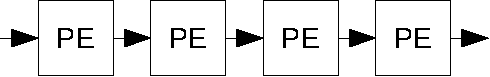
\includegraphics[scale=.5]{images/pipeline.pdf}
    \vspace*{1.15cm}
    \caption[]%
    {{\small Pipeline}}
    \label{fig:pipeline}
  \end{subfigure}
  %\hspace*{\fill}
  \begin{subfigure}[b]{0.475\textwidth}
    \centering
    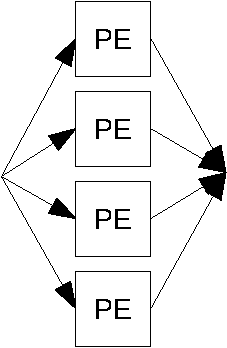
\includegraphics[scale=.5]{images/parallel.pdf}
    \caption[]%
    {{\small Parallel}}
    \label{fig:parallel}
  \end{subfigure}
  \vskip\baselineskip
  \begin{subfigure}[b]{0.475\textwidth}
    \centering
    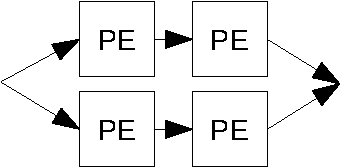
\includegraphics[scale=.5]{images/parallel-pipeline.pdf}
    \caption[]%
    {{\small Parallel pipeline}}
    \label{fig:parallel-pipeline}
  \end{subfigure}
  %\hspace*{\fill}
  \begin{subfigure}[b]{0.475\textwidth}
    \centering
    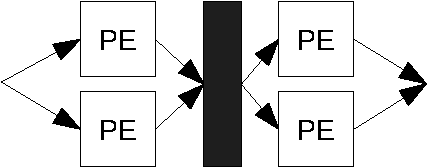
\includegraphics[scale=.5]{images/pipeline-parallel.pdf}
    \caption[]%
    {{\small Pipeline of parallel}}
    \label{fig:pipeline-parallel}
  \end{subfigure}
  \caption[]
  {\small Different processing element architectures}
  \label{fig:processing-element-organization}
\end{figure*}

The parallel configuration is typically used for higher layer networking applications, where as the pipeline configurations are used in line cards that require high-speed processing at low layer networking applications.

\section{Programming Models}

% \todo[inline]{Write a general view of the NPU programming models.}

Several generic software, development, and have been proposed to ease the development of high-speed packet processing applications for network processors.

% Different frameworks, such as Data Plane Development Kit~\cite{Intel:DPDK}, Open vSwitch~\cite{Pfaff:2009:OVS}, and Open Event Machine~\cite{OpenEM}, have been implemented to

\subsection{Data Plane Development Kit}
The Data Plane Development Kit (DPDK) provides a clean application programming interface and a set of coherent libraries and drivers, for Intel x86 processors. It has a generic support for many CPU's and network interface controllers ranging from Intel Atom processors to Intel Xeon processors. It supports system with and without non-uniform memory access (NUMA), and any number of processing cores.~\cite{Intel:DPDK:Doc}

DPDK runs as a Linux user-space application, utilizing the pthread library. Similarly to many other packet processing frameworks, DPDK implements a run-to-completion model, to minimize the process-switching overhead. The model removes the typical operating system scheduler. All the devices must be accessed by polling, thus eliminating the interrupt overhead. The packets can be passed between the cores, enabling more efficient and flexible core usage.~\cite{Intel:DPDK:Doc}

DPDK's Environment Abstraction Layer (EAL) abstracts the hardware environment from applications and libraries, enabling hardware agnostic implementation of packet processing applications. EAL provides services such as core affinity and assignment procedures, memory management, atomic and lock operations, and bus accesses, and interrupt handling. These features are exposed as a programming libraries.~\cite{Intel:DPDK:Doc}

DPDK has an active ecosystem around it, with wide vendor support. It is also well documented and includes several software examples demonstrating the best practices for data plane architectures, application profiling, and performance tuning.~\cite{Intel:DPDK:Doc}

\subsection{Open Event-Machine}
Open Event Machine (OpenEM) is an event-driven programming framework for multicore dataplane applications, developed by Nokia Solutions and Networks (NSN). It has been designed to ease the implementation of event/packet processing applications for different MPSoC devices. One of main drivers for the development of OpenEM has been easy integration with modern hardware accelerators.

The key concepts of OpenEM framework are execution objects, events, queues, and the scheduler. \emph{Execution objects} are the main building blocks the OpenEM application. They are the run-to-completion functions, describing the processing logic of the application. Each execution object has one or more \emph{queues} attached to it. The \emph{scheduler} selects the events from the queues, based on the global interrelations of the queues. When the event is selected from the queue, the corresponding execution object is attached to the processing core, and the event is passed to it as a parameter. Once the execution object finishes its run, the scheduler chooses a new event from the queues similarly.

From the programmer's perspective, OpenEM's event-driven programming model relates closely to actor based programming models such as Erlang~\cite{Armstrong:1993:Concurrent} and Akka framework~\cite{Akka}. While the use cases for these frameworks are completely different, and thus cannot directly be compared with OpenEM, it is worth mentioning their message passing support. Support for combined inter-node and intra-node parallelism has potential benefits for efficient scaling in the future. HCMPI~\cite{Chatterjee:2013:HCMPI} is an example of experimental framework that combines task-parallelism with message passing. OpenEM's current specification does not support inter-node messaging.

\section{Cavium OCTEON II CN6880}
\label{sec:cavium-octeon}
%https://www.reddit.com/r/networking/comments/2kamp1/eli5_why_are_cavium_chipsets_so_popular_with
Cavium Octeon II CN6880 is a network processing unit, optimized for high-performance, high-bandwidth, and low power consumption software-defined control-plane and data-plane applications.

CN6880's ingress and egress processing are handled by separate processing elements. The packet input processor unit (PKI) and input packet data unit (IPD) work together to manage the received packets, and to perform required processing before scheduling the packets to application cores. Once the required ingress computation is done, the PKI unit sends the packet's work entry to the SSO unit to be scheduled for processing.~\cite{cavium:2010:fundamentals}

The egress functions are handled by the packet transmission unit (PKO). When a core finishes a packet processing, it notifies the PKO that the packet is ready for transmission. The PKO then directly copies the packet data from the shared memory into its internal memory, optionally computes checksums for the packet header, transmits the packet, and optionally frees the packet data from the memory.~\cite{cavium:2010:fundamentals}

CN6880 consists of 32 MIPS application cores, with several hardware acceleration units for enhanced packet processing and minimized software development complexity. The packet management accelerators offload the actual packet processing cores from many general packet receive, buffering, buffer management, flow classification, quality of service, and transmit processing. The accelerator functions can be customized using software, and accessing the configuration registers. Together with the hardware acceleration units, the processing cores can handle most of the processing requirements of all the way through layer 2 to layer 7 in the standard OSI model~\cite{ISO:1994:OSI}.~\cite{cavium:2010:fundamentals}

One of the key features of the CN6880 is its scheduling/synchronization and order unit (SSO). It frees the actual packet processing applications, running on the 32 MIPS cores, from the complex packet scheduling and ordering tasks. The cores execute a loop, and when a core is ready for the next packet, it requests work from the SSO, which then schedules the next work based on the quality of service priority and work group.~\cite{cavium:2010:fundamentals}

The SSO has efficient locking mechanisms for protecting the critical regions without explicit software locking, and allows packet processing to be done in parallel or atomically, while still maintaining the packet flow order. The processing cores can also be dedicated for specific flows. One of our goals is to be able to model the scheduling functionality with PSE, as it is one of the key elements in the packet latency and throughput when processing several flows at the time.~\cite{cavium:2010:fundamentals}

% The memory latencies have large effect in the packet processing times.

The CN6880 provides several memory policies for optimized multi-core packet processing. Each of the 32 cores have dedicated 32KB L1 data and 37KB L1 instruction cache, and a shared 4MB L2 cache. The L1 data cache provides a hybrid write-through, write-back policy, using a write buffer mechanism, and the L2 cache implements a write-back policy. Several other cache related features are offered, for example to avoid unnecessary data writes after the packet transmission, and to automatically send the received packet header to L2 cache and the packet data to main memory, bypassing the L2 cache.~\cite{cavium:2010:fundamentals}

\section{Characteristic Measurements}
\label{sec:characteristic-measurements}

For the model to represent the packet latencies and throughput with enough accuracy, the model needs to be filled with apposite entity parameters. Some of the model parameters are simple enough to be obtained directly from~\cite{cavium:2010:fundamentals}, while others are either unavailable, or are presented in an unusable form to be used in the simulation model. The missing communication and memory related parameters are obtained by conducting measurements on the real CN6880 hardware. These are discussed in the following sections, respectively.

% We believe that, by determining the latecies of input phase and output phase, the behavior of memory, and modeling the packet scheduler with enough accuracy, the sought applications' effects to the packet latencies and throughput come up with enough accuracy.

% For our approach to be valid, i.e. the abstraction of the communication latencies to be precise enough, we have to assume the fastpath is not the bottleneck in the processing phase. This assumption is reasonable because ...

% \fixme{
%   TODO:
%   \begin{itemize}
%   \item because the fastpath hardware is optimized for this task
%   \item find reference
%   \item maybe justify the stuff with some kind of rough back-of-the-envelope calculation?
%   \end{itemize}
% }

\subsection{Communication Latencies}
\label{sec:communication-latencies}

By communication latencies, we refer to the time in the input and output phase of the packet processing, between physical receive/transmit ports and the actual core processing, as described in the Section~\ref{sec:cavium-octeon}. We will include the times spent in the SSO unit for both of these metrics, as due to our resource constraints, we were unable to do the measurements with the required detail to break down these delays. Also, for our modeling purposes, it is accurate enough to assume that the input and output phases consume equal amount of processing time.

The input and output phase latencies are measured by generating traffic from external machine, and passing it through two CN6880 units back to the generator itself. The measurements were done at two independent points in the processing path, to validate the accuracy of the measurements.

\begin{figure}[]
  \begin{center}
    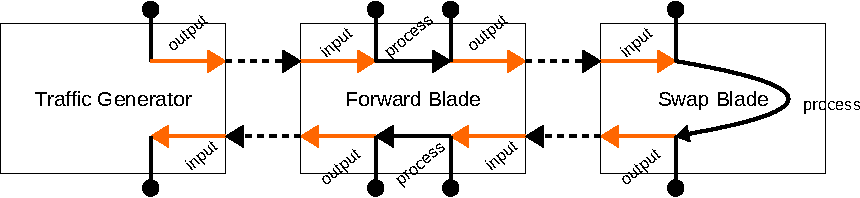
\includegraphics[width=\textwidth]{images/comm-measurement-setup.pdf}
    \caption{The setup used to measure the communication latencies. The communication between the nodes, packet processing on the main cores, and the input and output processing, are marked with the dashed arrows, solid black arrows, and orange arrows respectively. The probes present the points of measurement.}
    \label{fig:comm-setup}
  \end{center}
\end{figure}

In Figure~\ref{fig:comm-setup}, the rectangles represent three different computing units (traffic generator, forward unit, and swap unit), and the probes present the points of time measurements. The traffic generator is a typical desktop computer running Ubuntu operating system, and the traffic was generated by Mausezahn~\cite{mausezahn}. Both of the Octeon CN6880 units are running Linux operating systems.

The packet is first generated at the packet generator and sent to the forward unit at time $t^{d}_{0}$. Forwarding unit receives the packet at time $t^{r}_{10}$, does the required processing and forwards the packet to the swap unit at time $t^{d}_{10}$. The swap unit receives the packet at time $t^{r}_{2}$, does the same processing as the forward unit (except with different destination address), and forwards the packet back to the forward unit at time $t^{d}_{2}$. Finally the forward unit receives the packet at time $t^{r}_{11}$ and forwards it to the traffic generator at time $t^{d}_{11}$, which marks it received at time $t^{r}_{0}$. The time $t_{f}$ spent in the input and output phase of one unit is then

\begin{equation}
  \label{eq:1}
  t_{f} \approx \frac{t^{r}_{11} - t^{d}_{10} - (t^{d}_{2} - t^{r}_{2})}{2}.
\end{equation}

We measured the times for packet sizes of 64B, 128B, 256B, 512B, 1024B, and 1500B, repeating the measurement for each packet 10000 times. Figures~\ref{fig:comm-latency-boxplot} and~\ref{fig:comm-latency-histograms} present the statistics of the resulting times $t_{f}$ for the different packet sizes.

\begin{figure}[]
  \begin{center}
    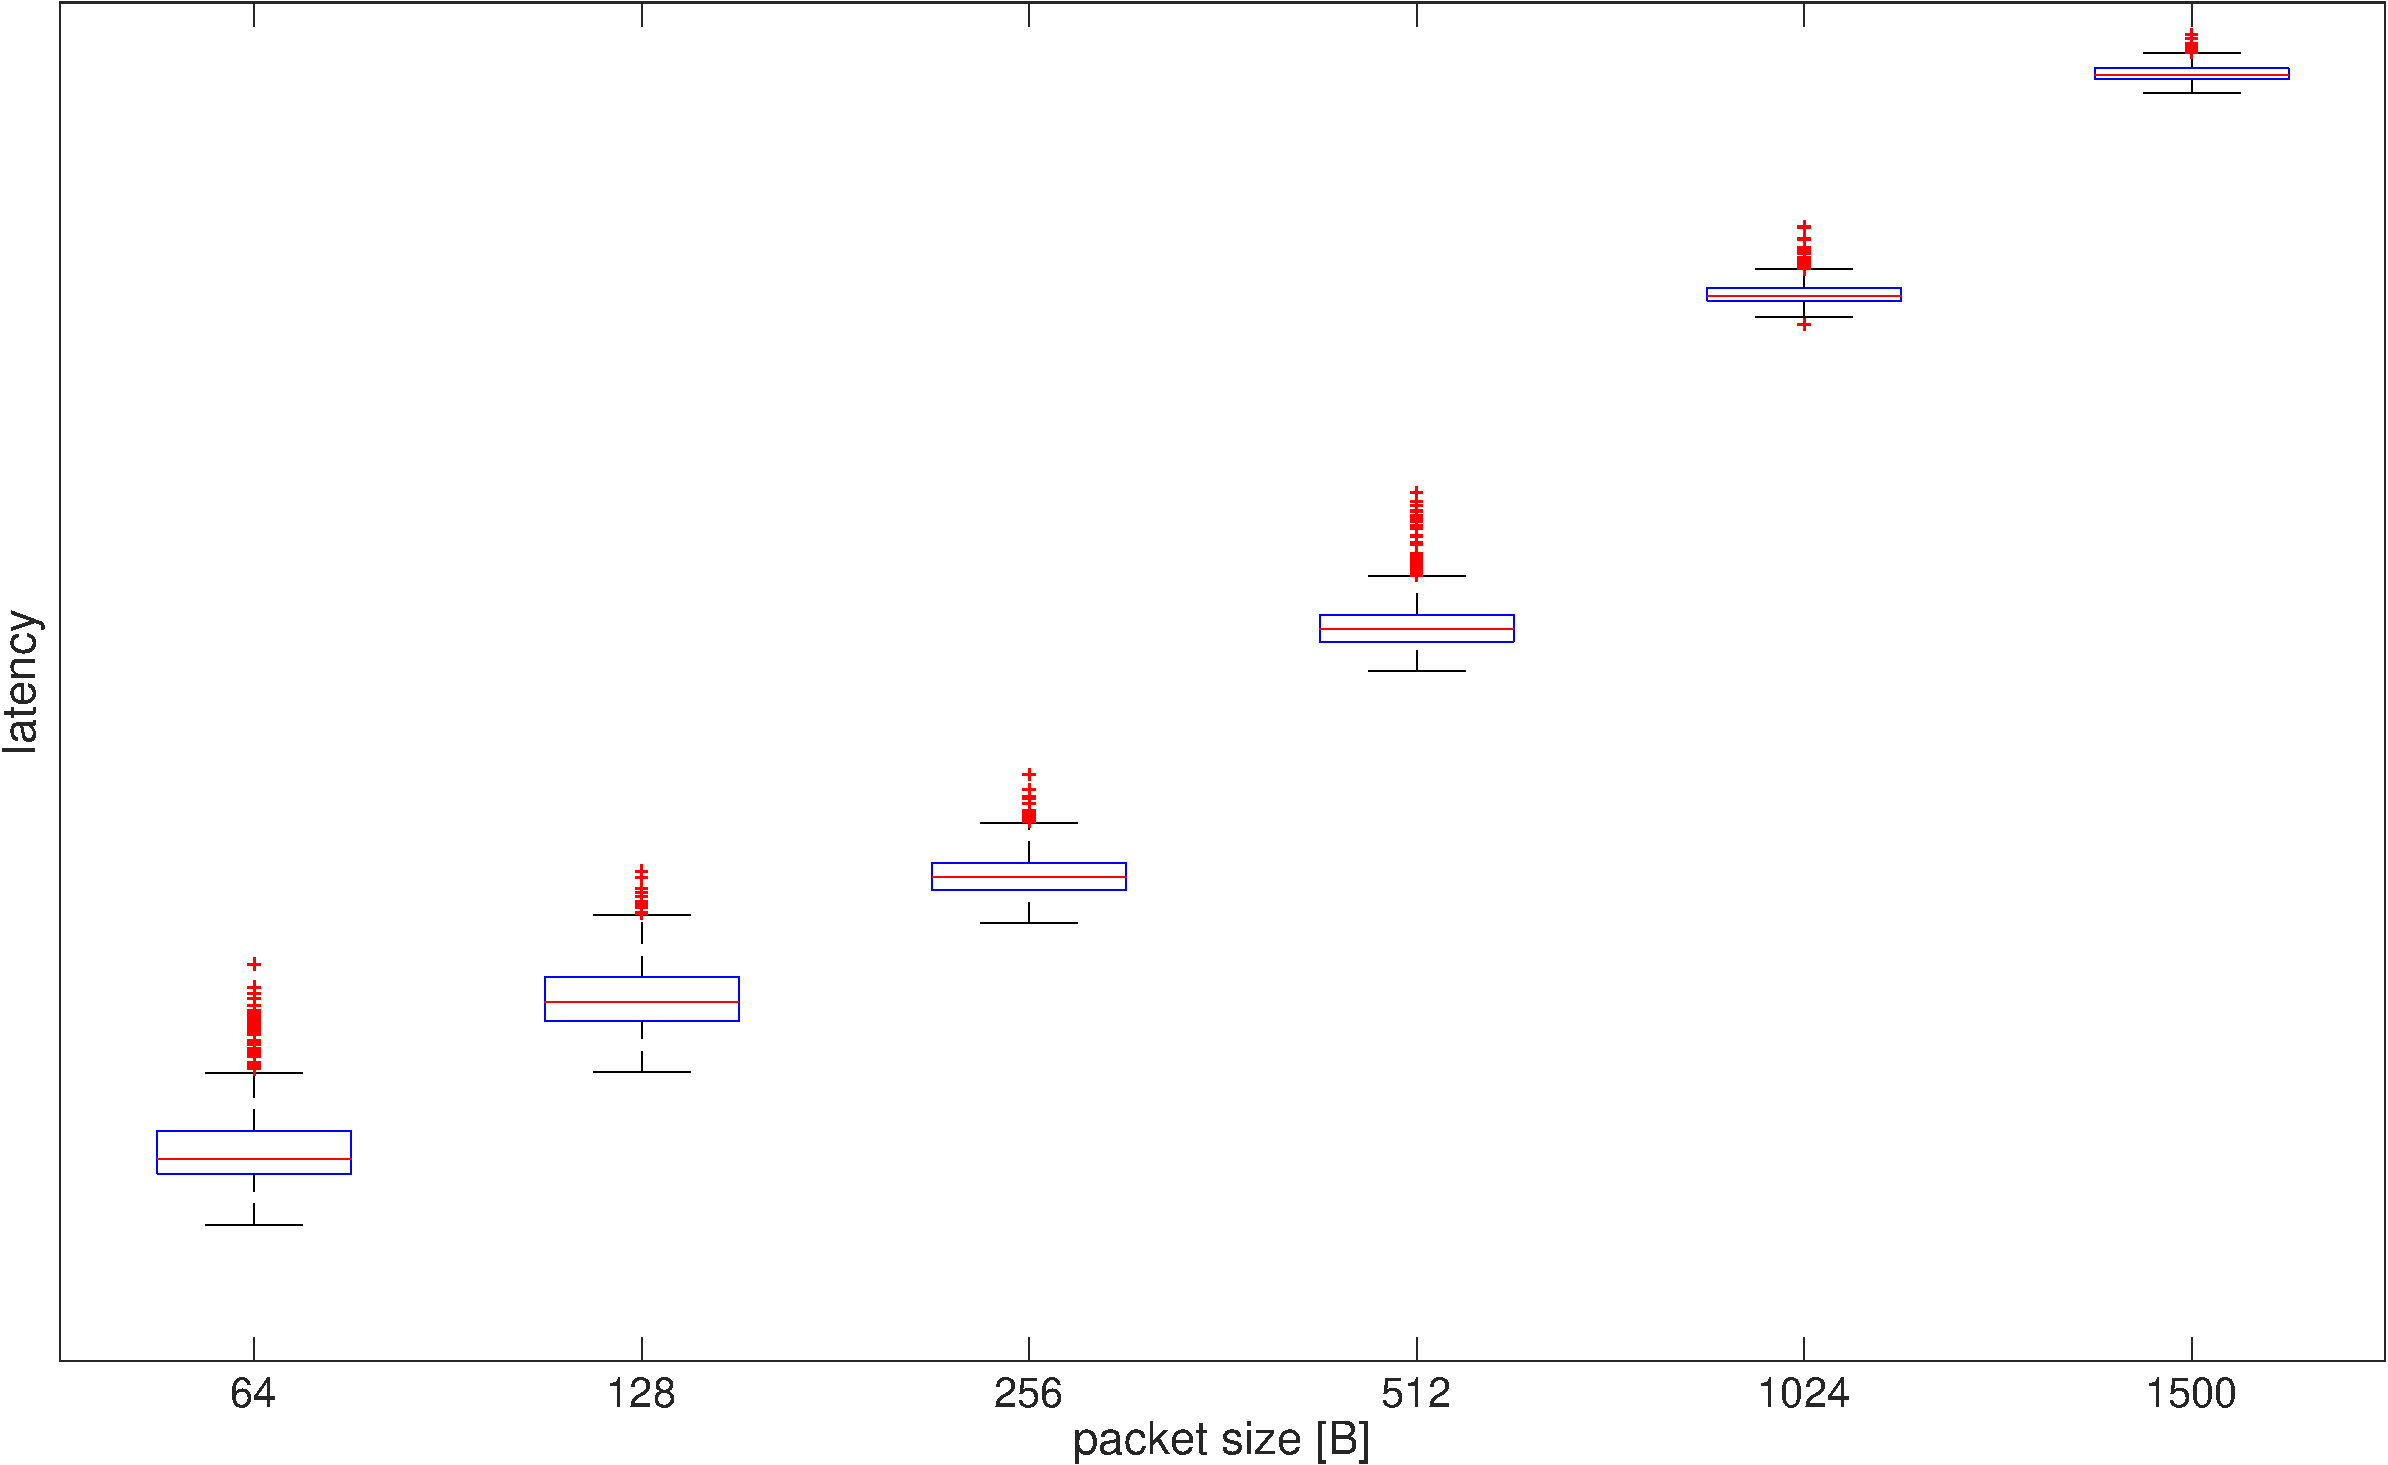
\includegraphics[width=\textwidth]{images/comm-latency-boxplot.pdf}
    \caption{Latency of the input and output phase of the CN6880 unit. On each box, the central mark is the median, the edges of the box are the 25th and 75th percentiles. 99.3\% of the points lie within the whiskers, and the most extreme points are presented as red crosses. Both of the axes are on logarithmic scale.}
    \label{fig:comm-latency-boxplot}
  \end{center}
\end{figure}

\begin{figure}[]
  \begin{center}
    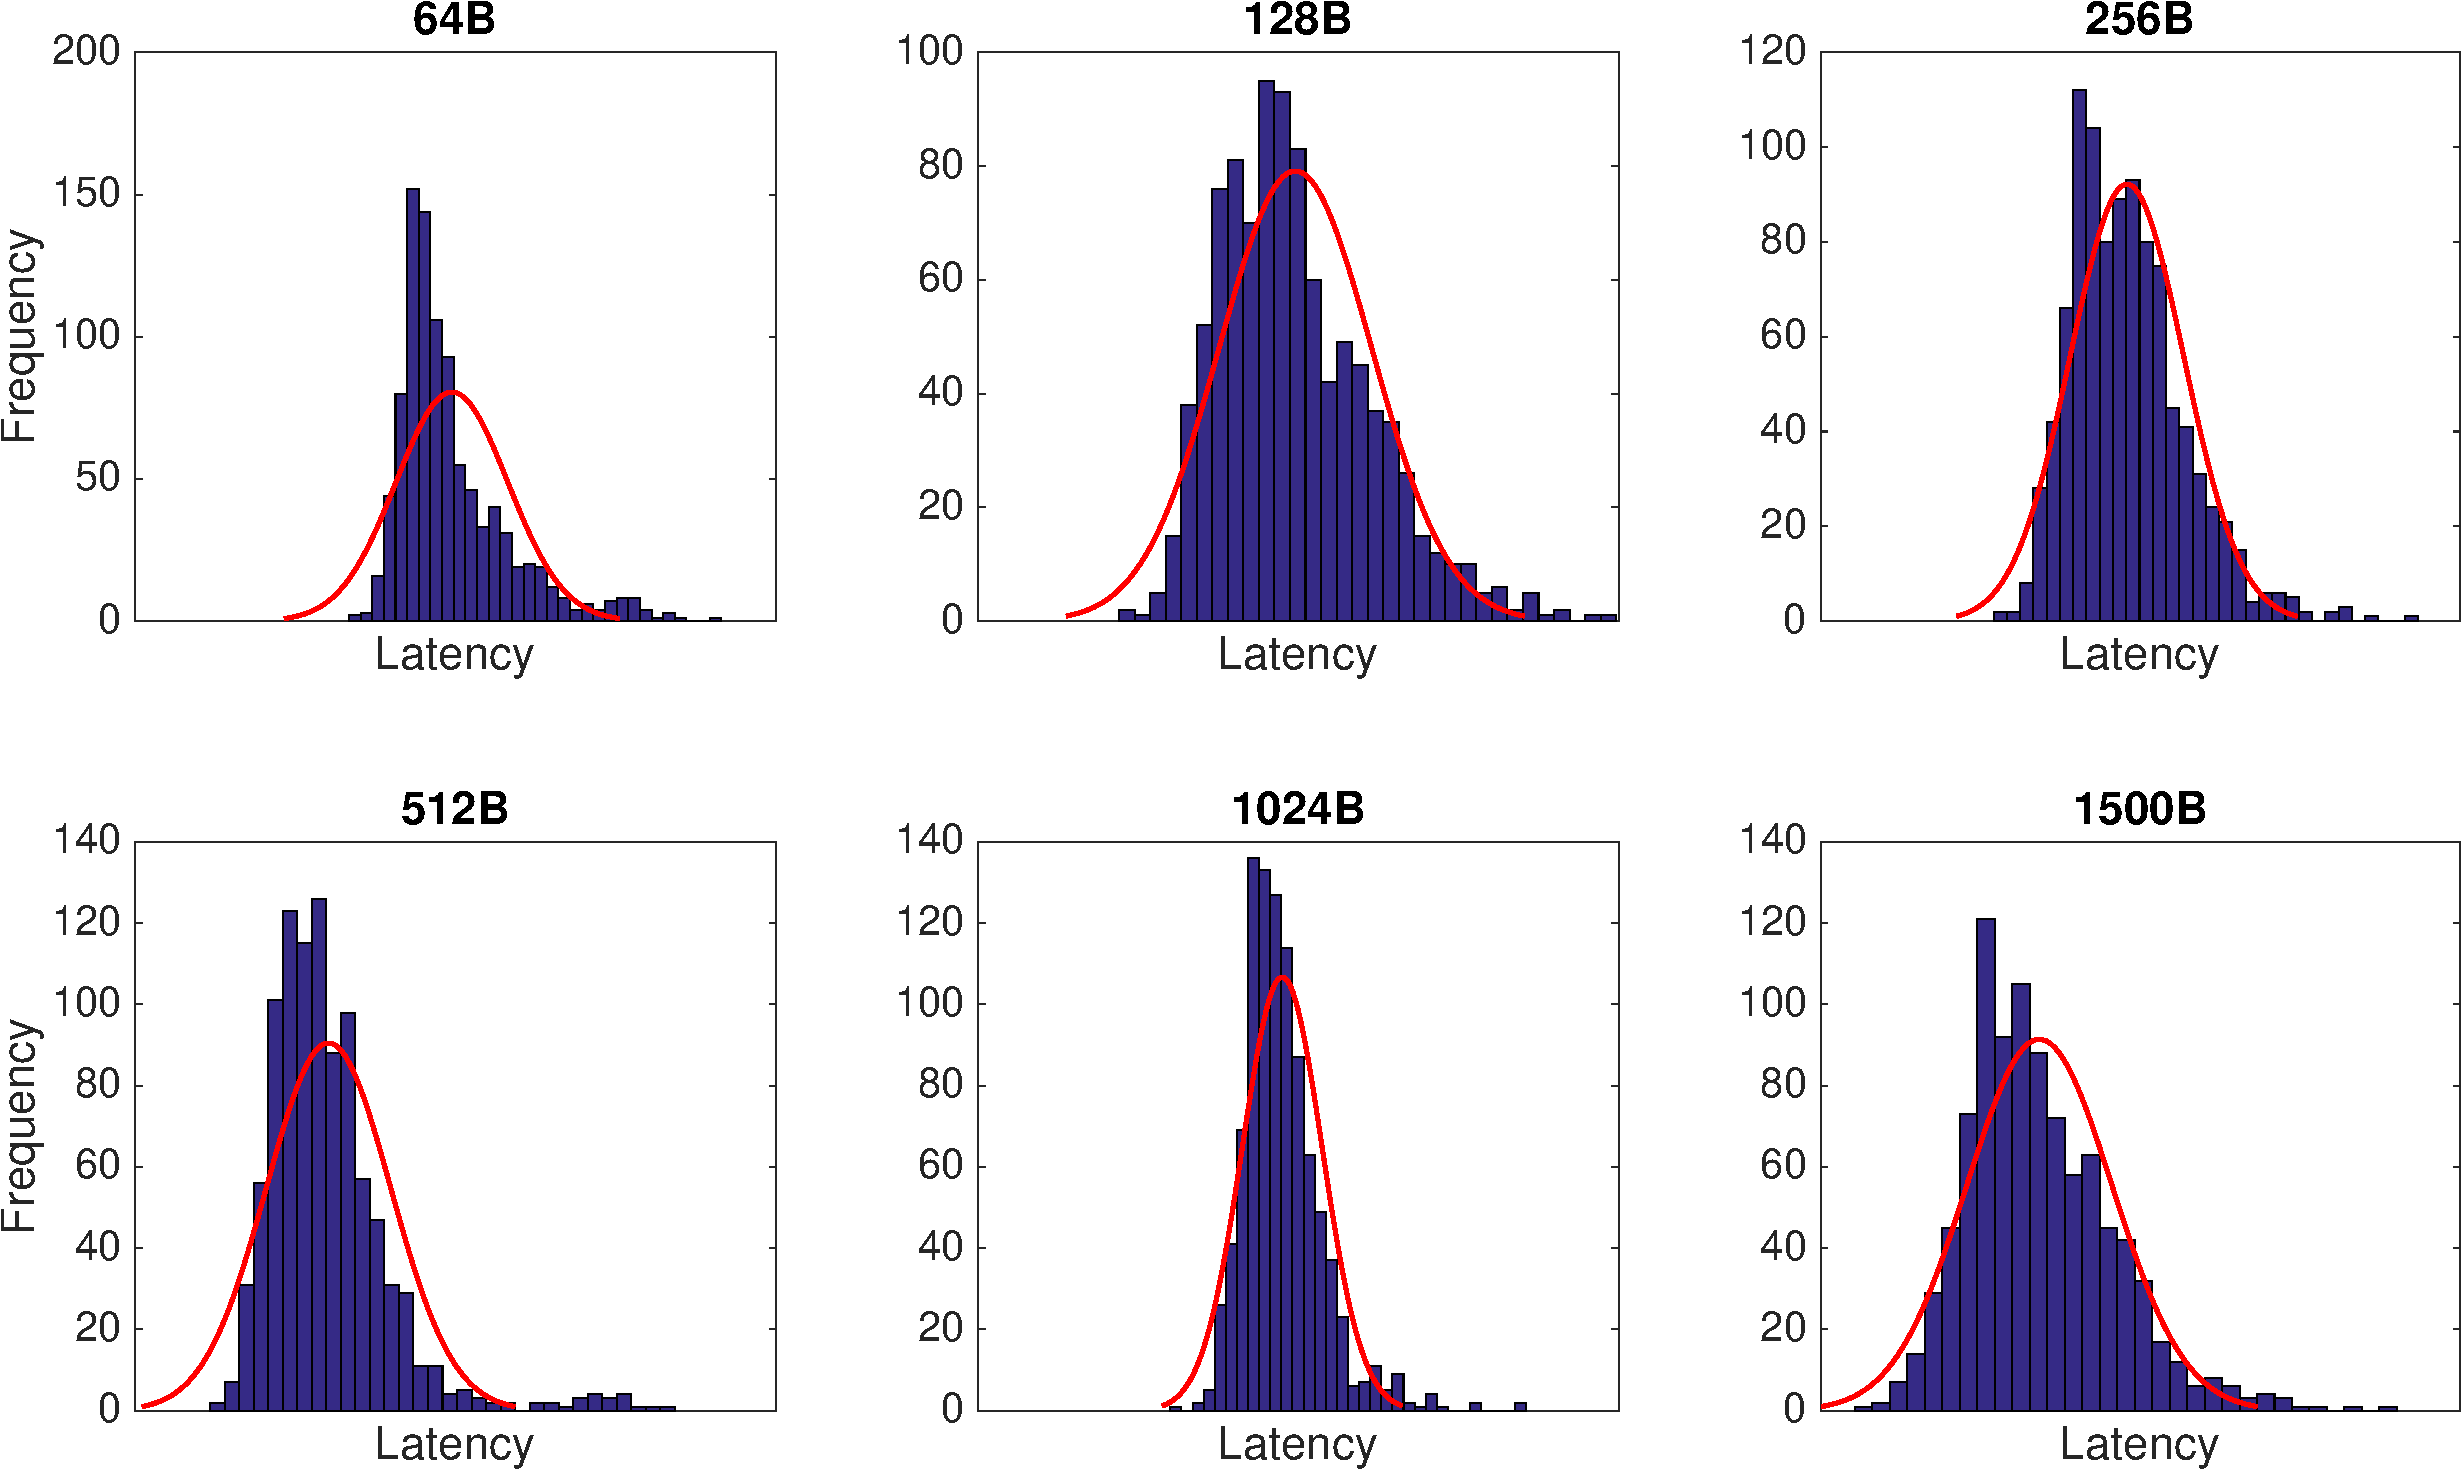
\includegraphics[width=\textwidth]{images/comm-latency-histograms.pdf}
    \caption{Latency frequency histograms for each packet size, along with a normal density function with parameters, estimated with maximum likelihood method from the data.}
    \label{fig:comm-latency-histograms}
  \end{center}
\end{figure}

As shown in the Figure~\ref{fig:comm-latency-boxplot}, the time spent in the input and output phase of the unit is roughly linear regarding to the packet size. The variation of the data is relatively small on all packet sizes. The trend of the latency with respect to the packet size, corresponds to the trend of the values measured with at the external traffic-generator (which causes $3.1\mu s$ constant overhead regardless of the packet size). The corresponding plots for the external traffic-generator measurements are omitted for clarity.

As seen from both of the Figures~\ref{fig:comm-latency-boxplot} and ~\ref{fig:comm-latency-histograms}, there exist points with unexpectly large deviation from the rest of the group. These deviations seem to be independent of the packet size, and thus we assume that they are caused by the scheduling unit (SSO). This behavior is also statistically incorporated in the simulation model.

The only packet size dependent operations in the input and output phases are the memory transfers done for the actual packet data between the memory (L2/RAM) and PKI or PKO. All the other other operations are done based on the packet header, thus requiring constant amount of time regardless of the packet size.

Since We cannot make a distinction between the input and output phase, in the simulation model presented further, we will adjust the input/output phase amount so that they consume the PKI and PKO units for the amount that corresponds the constant term of equation~\ref{eq:1}. The variable (non-constant) term is caused by the memory copies in the input/output phases, and are proportional to the packet size.

The input and output delays used in the simulation model are estimated by fitting a linear model to the data, using least square estimate. The determination coefficient of the estimate $R^2 = 0.997$. The delay for the input and output phase are divided evenly, resulting in

\begin{equation}
  \label{eq:1}
  t_{in} = t_{out} = \frac{1}{2}(0.0018\frac{\mu s}{B} * packet\_size + 1.036\mu s).
\end{equation}

\subsection{Memory Characteristics}
\label{sec:memory-characteristics}

Memory delays were measured using Multi-core Processor Architecture and Communication (MPAC) benchmarking library~\cite{Jamal:2009:MPAC}. Both, latency and throughput were measured using different dataset sizes and number of threads. Each the tests was run with 200,000 repetitions.

\begin{figure}[]
  \begin{center}
    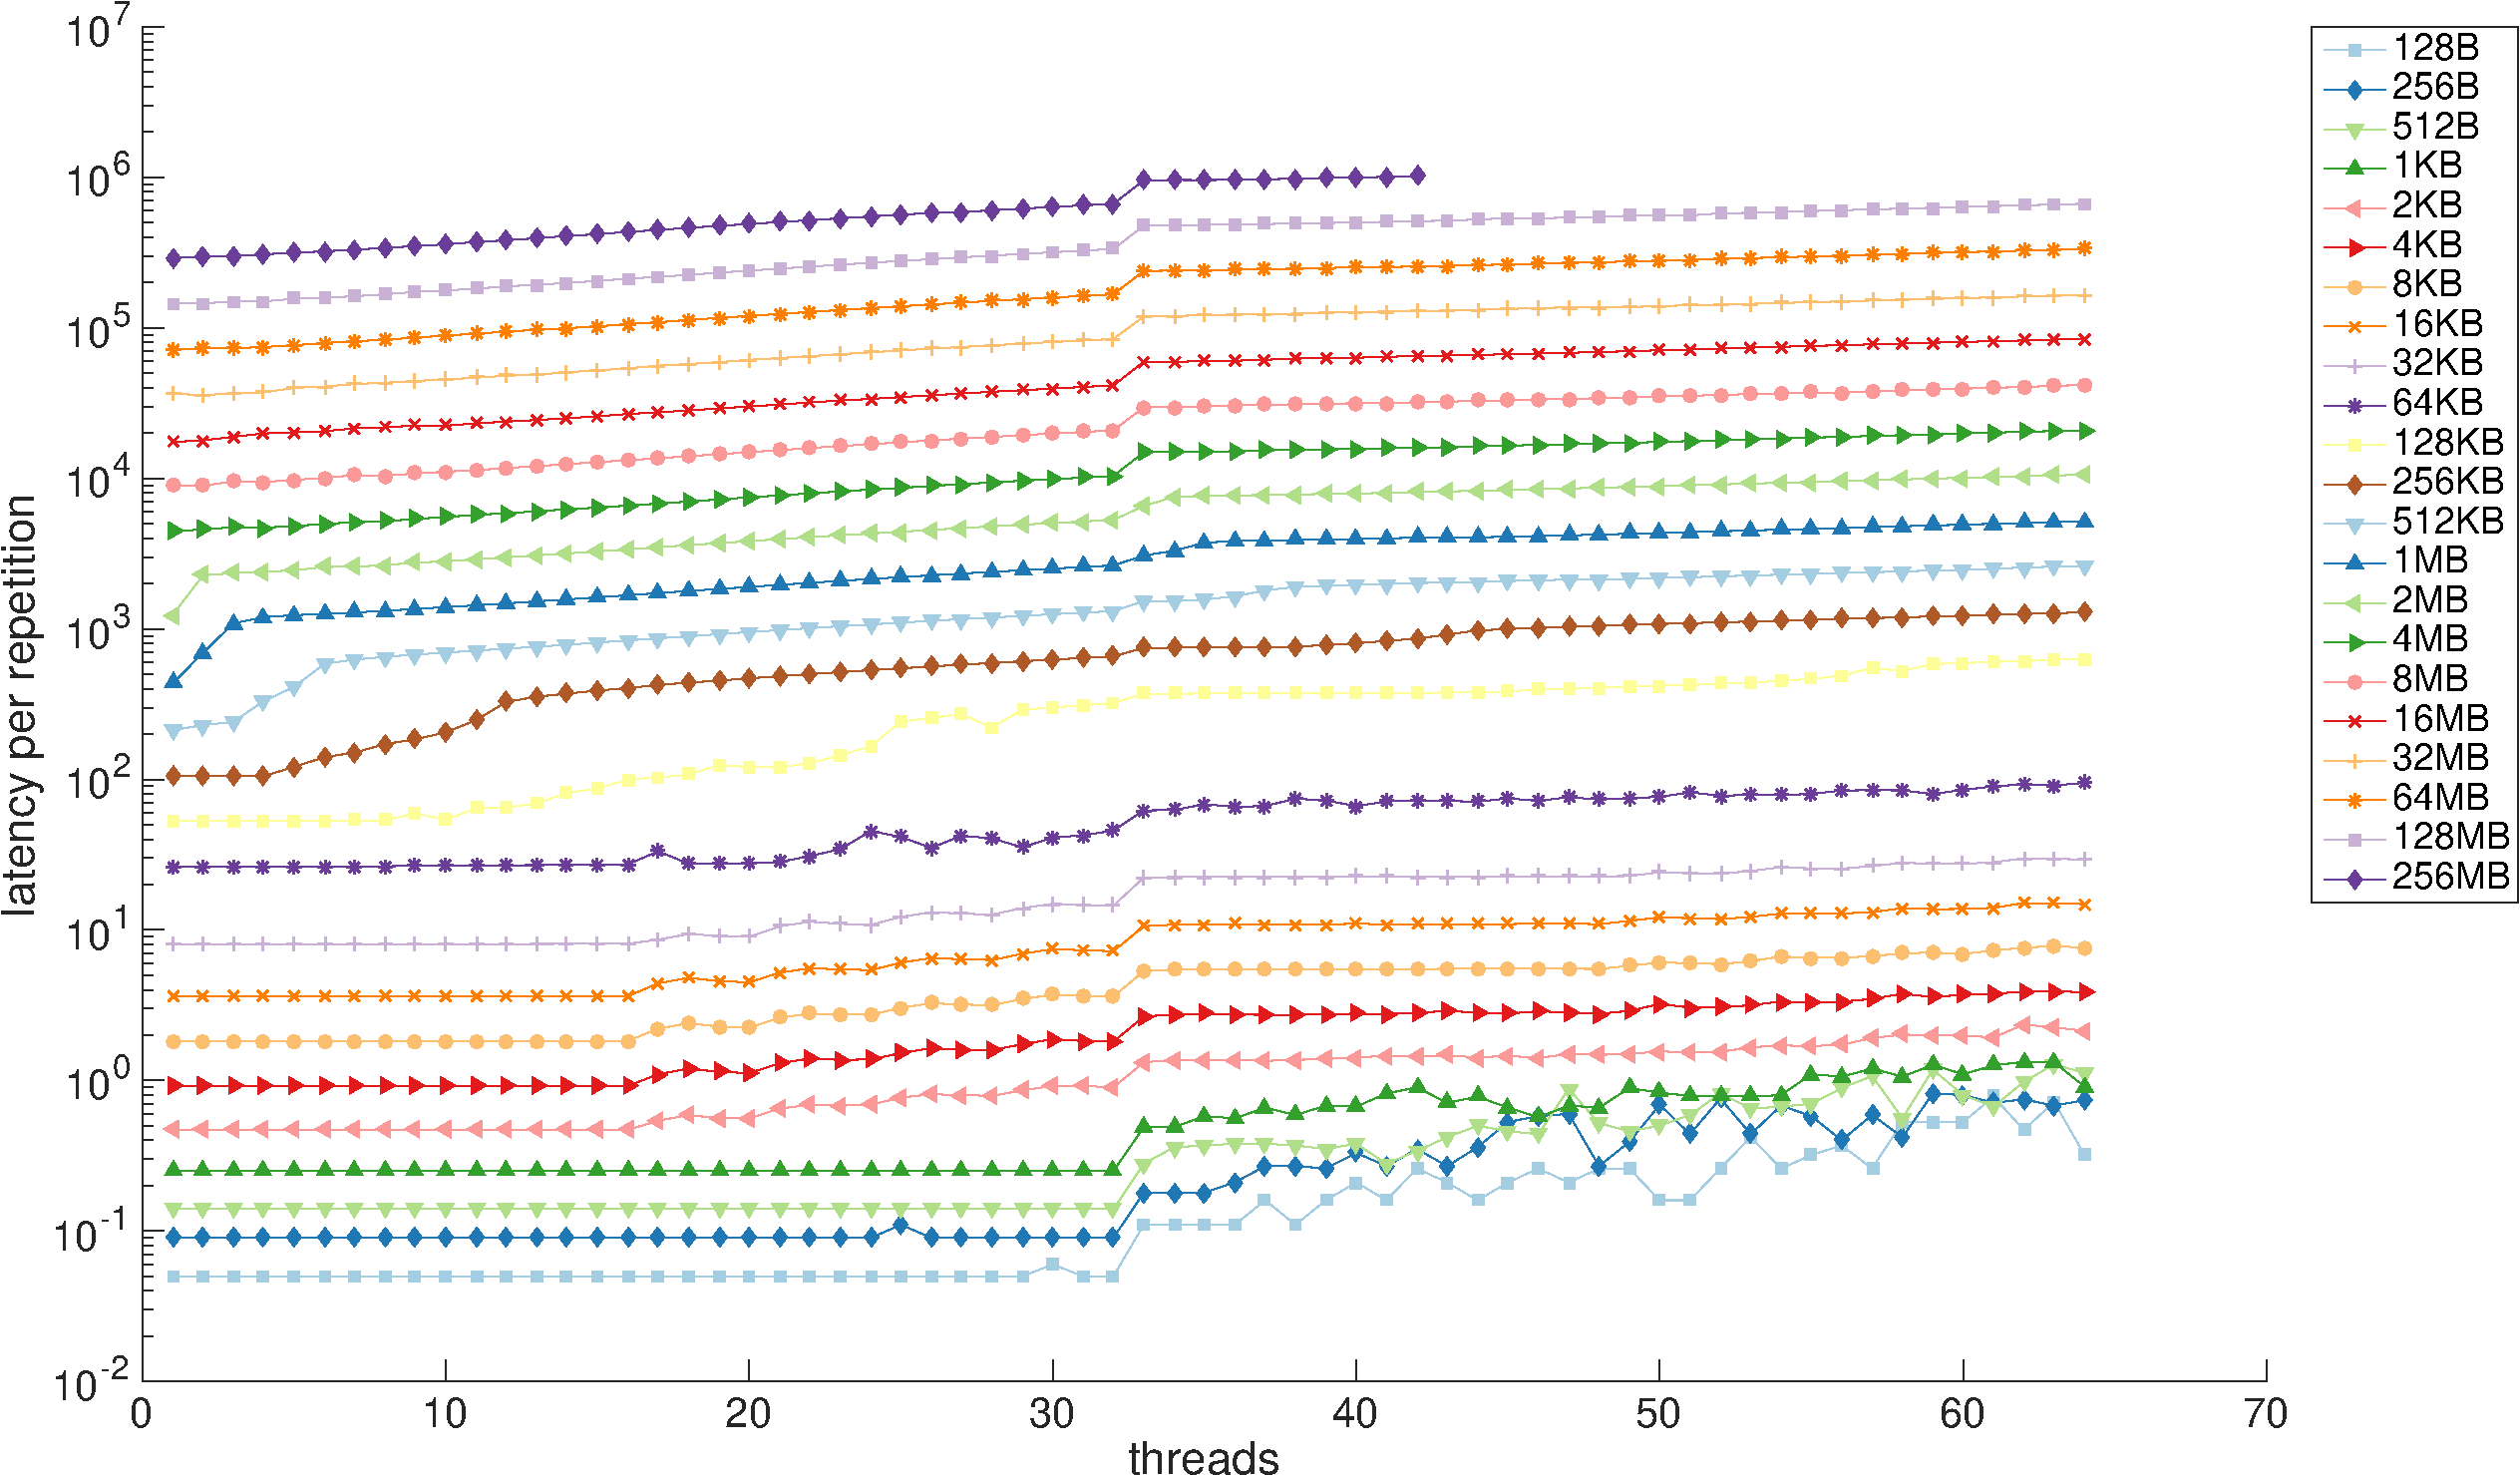
\includegraphics[width=\textwidth]{images/mem-latency.pdf}
    \caption{Memory latency of the CN6880 in microseconds across number of threads for integer data type (32bit), measured by MPAC. Each data point in the graph present one experiment run with different thread and write sizes. The latencies for different packet sizes are marked with colors as shown in the legend (in bytes). The y-axis is presented in logarithmic scale.}
    \label{fig:mem-latency}
  \end{center}
\end{figure}

Figure~\ref{fig:mem-latency} presents the results from the latency measurements for different packet sizes and thread counts. Notice that the y-axis the graph is logarithmic. As expected, the memory latencies grow together with the size of the write. The transition between the memory levels (32K L1, 4MB L2~\cite{cavium:2010:fundamentals}) can be seen as the jumps in the latency graph. With 128B - 1KB write sizes both the read and write arrays fit in the L1 cache (32KB~\cite{cavium:2010:fundamentals}), and thus the latency per repetition is independent of the thread count. With write sizes above 2KB, some of the writes hit L2 cache (4MB~\cite{cavium:2010:fundamentals}), increasing the latency as the thread count increases. Similarly, the step from L2 cache to RAM can be seen 128KB, 256KB, 512KB, 1MB, and 2MB write sizes, where both write and read arrays completely fit in the L2 cache with 8, 4, 2, 1 and 1 threads, and move to RAM beyond that.

The write latencies also thrash beyond 32 threads, especially for the cache sizes. This does not affect the main core memory accesses in the model, as only 32 threads are used for packet processing. However, these numbers work as a reference when modeling the memory communication of other units such as SSO.

\begin{figure}[]
  \begin{center}
    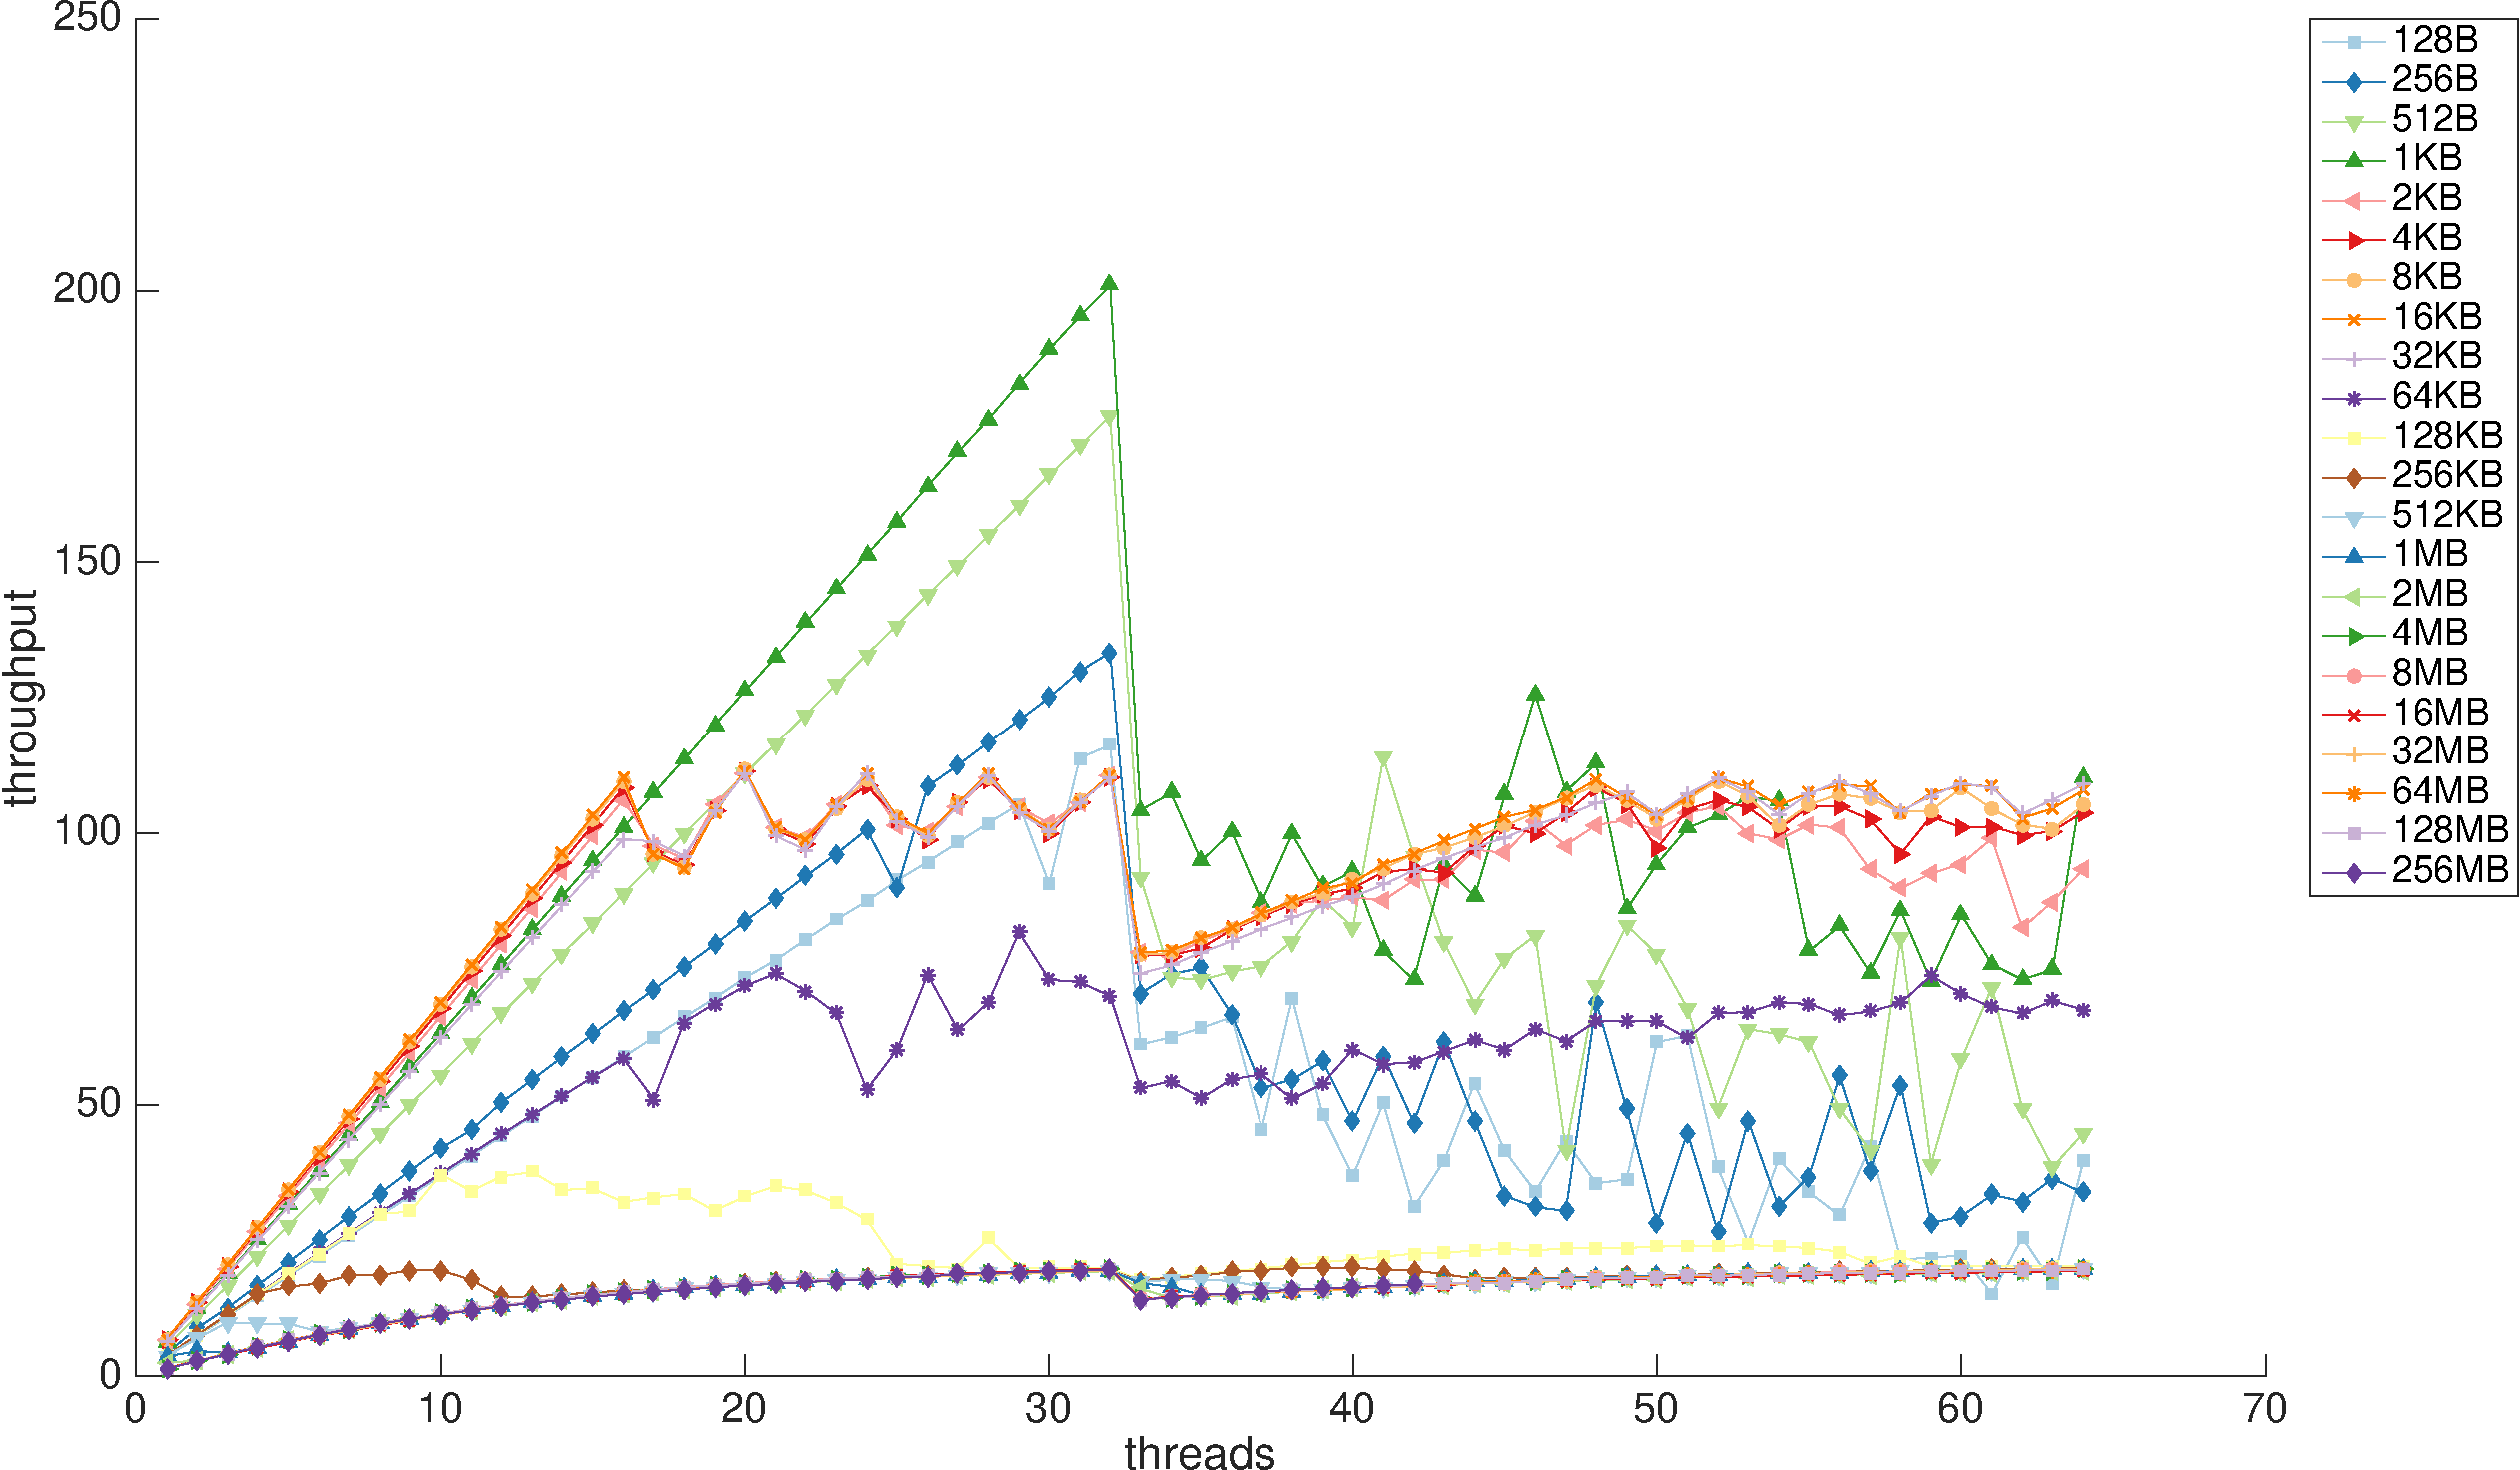
\includegraphics[width=\textwidth]{images/mem-throughput.pdf}
    \caption{Memory throughput of the CN6880 in Gbps across number of threads for integer data type (32bit), measured by MPAC. Each data point in the graph present one experiment run with different thread and data sizes. The throughput for different packet sizes are marked with colors as shown in the legend (in bytes).}
    \label{fig:mem-throughput}
  \end{center}
\end{figure}

Figure~\ref{fig:mem-latency} presents the results from the throughput measurements for different packet sizes and thread counts. Again, as expected, the maximum throughput is achieved with 1KB write lengths and 32 cores, when both the write and read arrays fit in the caches. The write throughput scales linearly with 128B - 1KB write sizes for up to 32 cores, with 2KB - 64KB up to 16 cores, and for 256KB, 512KB, and 1MB, write sizes up to 8, 4, and 2 cores respectively. The transitions between the memory levels are similar as in the latency graph. Again, a clear thrashing can be seen with more than 32 threads.


%%% Local Variables:
%%% mode: latex
%%% TeX-master: "thesis-hartikainen"
%%% End:
